\chapter{Results}
To validate the CUE model, I matched it against human experimental data of serial and free recall experiments.
The same model architecture was used in all of these simulations with only small changes in some parameter values across experimental conditions.
The simulations were designed to replicate the experimental paradigms as closely as possible.
In particular, the list length, item presentation times, delay times, and recall times were matched.

To model the effect of distractor tasks during delay phases, non-list items where presented a rate of $\drate$ items per second.
These were allowed to influence the STM component, but learning in the LTM component was disabled as these items were irrelevant to the main memorization task.
This is similar to how \textcite{Howard2002} modeled the distractor interval, though in their case they did not define the distractor rate, but the effective length of the distractor interval.
As I was aiming to match the experimental paradigms as closely as possible, changing the length of the distractor interval was not an option.

Unless otherwise noted, 100 simulations with different seeds were run per experimental condition.
This number is sufficient to get clear results with reasonably small confidence intervals, but still small enough that the simulation and parameter matching is feasible on a high-performance computing cluster.
The values used for free parameters in the different settings are summarized in \cref{tbl:params}.
In addition to these, the context drift parameter was set to $\tcmbeta = 0.62676$ and the OSE short term decay was set to $\osestmdecay = 0.9775$ in all simulations.
These are the values reported as best fitting by \textcite{Sederberg2008} and \textcite{Choo2010} respectively.
Some other parameters, like the OSE scaling $\oseepisscale$ for episodic memory and the TCM ratio $\gamma$ for updating $\mft$, are not present in the CUE model.
\begin{table}
    \centering
    \caption[Summary of free parameter values]{Summary of free parameters values for distractor rate $\drate$, probability $\psi$ of using the serial recall strategy in free recall, bias of the null choice $\minev$ in recall, standard deviation of the input noise $\recnoise$ in recall, and the AML learning rate $\eta$.}\label{tbl:params}
    \begin{tabular}{lSSSSS}
        \toprule
        Experimental condition & $\drate / \si{\second^{-1}}$ & $\psi$ & $\minev$ & $\recnoise$ & $\eta$ \\
        \midrule
        \textbf{Serial recall} & & & & & \\
        \hspace{1em}Immediate & {\textemdash} & 1 & 0.04 & 0.009 & 10 \\
        \hspace{1em}w/o STM & {\textemdash} & 1 & 0.04 & 0.009 & 10 \\
        \hspace{1em}w/o LTM & {\textemdash} & 1 & 0.03 & 0.015 & 10 \\
        \textbf{Free recall} & & & & & \\
        \hspace{1em}Immediate & {\textemdash} & 0.1 & 0.04 & 0.015 & 10 \\
        \hspace{1em}Delayed & 0.4 & 0 & 0.0325 & 0.015 & 10 \\
        \hspace{1em}Continuous distractor & 0.3 & 0.1 & 0.03 & 0.009 & 10 \\
        \textbf{Scopolamine} & & & & \\
        \hspace{1em}Placebo & {\textemdash} & 0.1 & 0.02 & 0.015 & 10 \\
        \hspace{1em}Scopolamine & {\textemdash} & 0.1 & 0.02 & 0.015 & 0.1 \\
        \bottomrule
    \end{tabular}
\end{table}

\section{Serial recall}
In serial recall participants are asked to recall items in the same order as they were presented.
In an experiment presented by \textcite{Jahnke1968}, lists of ten items were presented at the rate of one item per second and recalled immediately.
\Cref{fig:results-serial} shows the serial position curve for the experimental and model data and the distribution of transposition errors averaged over all serial positions.
In both cases the serial position curve shows a clear primacy and recency effect.
The model predictions are statistically indistinguishable from the human data as all confidence intervals overlap.
While \textcite{Jahnke1968} did not provide the transposition data, the model qualitatively matches the transposition gradients reported elsewhere \parencite[e.g.,][]{Henson1996}.
In general, few transposition errors are made, but for those that occur, transpositions of nearby items are more likely than transpositions of distant items.
\begin{figure}
    \centering
    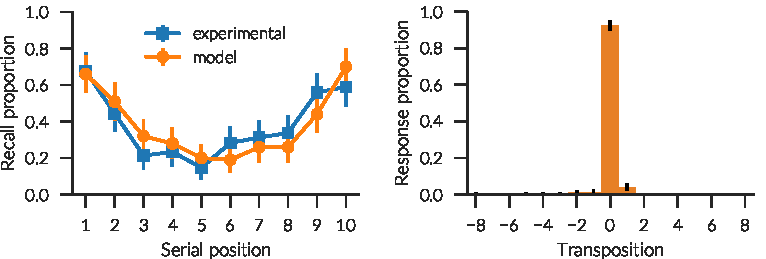
\includegraphics{figures/results/serial}
    \caption[Serial position curve and transpositions for serial recall with the CUE model]{Serial position curve (left) and transpositions (right) for the serial recall of a \num{10}~item list with the CUE model. The experimental data from \textcite{Jahnke1968} is shown for comparison in the serial position curve (blue squares). The error bars show \SI{95}{\percent} confidence intervals.}\label{fig:results-serial}
\end{figure}

The model allows selective disabling of the recall from the STM or LTM component.
Doing so, with appropriate adjustment of the recall noise level to account for the reduced evidence input, shows that the primacy effect is mediated by the LTM, while the recency effect depends on the STM (\cref{fig:results-no_xtm}).
The recall performance without the LTM contribution is also much worse.
This might be the case either because the input to the recall network might need further adjustment or because no rehearsal mechanism is modelled, resulting in drift of the OSE integrator.
\begin{figure}
    \centering
    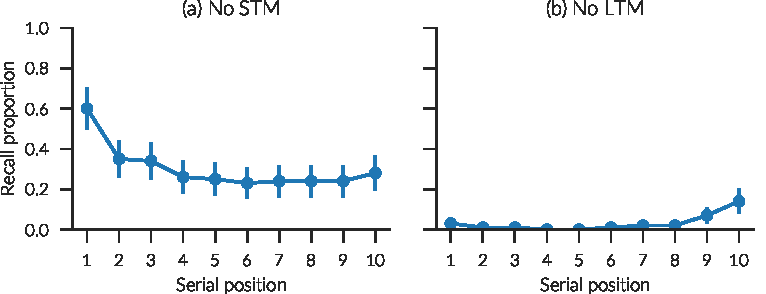
\includegraphics{figures/results/no_xtm}
    \caption[Serial position curves with disabled STM/LTM]{Serial position curves when either (a) STM recall or (b) LTM recall is disabled in the model.}\label{fig:results-no_xtm}
\end{figure}


\section{Free recall}
While the order of recall is predetermined in serial recall, in free recall list items may be recalled in any order.
Here, I provide the model match to the data from \textcite{Howard1999}, which has also been used in the original fits of the TCM model in \textcite{Howard2002} and \textcite{Sederberg2008}.
Three experimental conditions are matched: immediate recall, delayed recall, and continuous distractor recall.

In the immediate free recall condition, list items are presented at a rate of one item every second.
After the presentation phase, a recall phase of \SI{45}{\second} followed immediately.
This protocol is changed to a presentation rate of one item every \SI{1.2}{\second} and a recall phase of \SI{60}{\second} in the delayed and continuous distractor conditions.
In both of these latter conditions, the presentation and recall phase are separated by a \SI{16}{\second} distractor task.
In addition, in the continuous distractor conditions such a \SI{16}{\second} distractor phase is inserted in between every pair of items.
A list length of 12 items is used in all conditions.

Four resulting metrics from the model and experimental data are shown in \cref{fig:results-free}.
First, the distribution of the total number of successful recalls is shown.
To my knowledge, this data has not been analyzed for the original TCM model, even though it is arguably the most fundamental comparison.
In all conditions, the \SI{95}{\percent} confidence intervals of the mean, standard deviation, and kurtosis overlap with the exception of the kurtosis in the immediate recall condition.
Thus, no significant difference for the most essential moments is shown, which indicates that the model approximates the experimental distributions well, even though an equality of the distributions cannot be inferred.
\begin{figure}
    \centering
    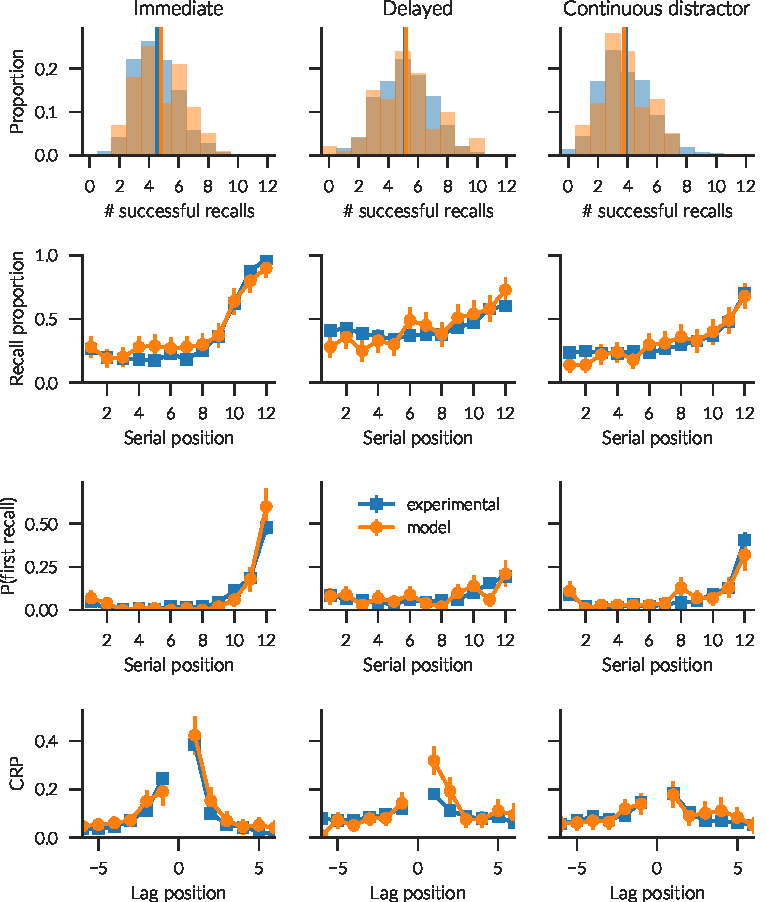
\includegraphics{figures/results/free}
    \caption[Comparison of experimental and model free recall data]{Comparison of experimental and model free recall data. The columns show data from the immediate, delayed, and continuous distractor conditions respectively. The rows show from top to bottom: distribution of the number of successful recalls (mean marked by vertical line), serial positions curves, probability of first recall, and the conditional response probability. The error bars show \SI{95}{\percent} confidence intervals. Experimental data by \textcite{Howard1999}.}\label{fig:results-free}
\end{figure}

Second, the serial position curves are given.
The strong recency effect in immediate recall is attenuated in delayed recall, but reappears to some degree in continuous distractor recall.
Interestingly, the recency effect in immediate recall gives the curve an S-like shape that is missing in continuous distractor recall.

Third, these effects also show in the probability of first recall.
In immediate recall, the first recall is, with high probability, from the end of the list, whereas in delayed recall the probability is much more uniform.
In continuous distractor recall, the probability to start the recall at the end of the list is partially restored.

Finally, the conditional response probability (CRP) gives the probability of how much lag there is between the positions of two recalled items is.
For example, the asymmetry in immediate recall shows the bias to do forward recall and the peak around zero that nearby items tend to be recalled together.
Both of these effects become attenuated in delayed and continuous distractor recall.
In delayed free recall, the model predicts a stronger forward bias than the experimental data shows.

The model provides an excellent fit on most measures.
The confidence intervals of \num{101} of the \num{108} data points overlap.
This amounts to less than \SI{7}{\percent} confidence intervals that do not overlap, while about \SI{5}{\percent} are expected to be non-overlapping by pure chance given a \SI{95}{\percent} confidence level.
The most salient deviation of the model and experimental data is observed in the CRP curve for the delayed recall condition.
The model predicts a slightly higher forward bias than is actually found.


\section{Scopolamine}
A spiking neural network model allows the investigation of the effects of drugs more readily than a pure mathematical model.
I demonstrate this here with the acetylcholine antagonist scopolamine.
Administered before the presentation phase in an immediate recall experiment, scopolamine is detrimental to recall performance \parencite{ghoneim1975}.
However, scopolamine administered in between the presentation and recall phase does not influence performance.
This indicates that scopolamine prevents encoding of new memories in LTM, but does not prevent recall of already encoded memories.
More precisely, scopolamine has been shown to attenuate long-term potentiation in hippocampus \parencite{leung2003,ito1988,hirotsu1989-1}.

To model the effect of scopolamine on LTP, A adjusted the AML learning rate for learning the $\mtf$ and $\mft$ matrices.
With this approach the experimental results by \textcite{ghoneim1975} are reproduced.
I focus here on the immediate recall experiment with Set~II\@.
% TODO explain Set II or delete
The simulation protocols were again modeled to replicate the experimental settings, with 16 items per list, and a presentation time of two seconds per item.
To obtain a similar effect, the normal AML learning rate was used before the time point of scopolamine injection and in placebo trials.
After the time point of scopolamine injection it was scaled set to zero.

\Textcite{ghoneim1975} reported a recall accuracy of \SI{77.92(494)}{\percent} (mean $\smash{\pm}$ standard error) in the placebo condition and a recall accuracy of \SI{31.67(228)}{\percent} in the scopolamine condition.
The model produces recall accuracies of \SI{74.18(108)}{\percent} and
\SI{37.94(99)}{\percent}
respectively.
Moreover, the serial position curve for the scopolamine condition shows no primacy effect, but a recency effect (\cref{fig:scopolamine-serial}).
\begin{figure}
    \centering
    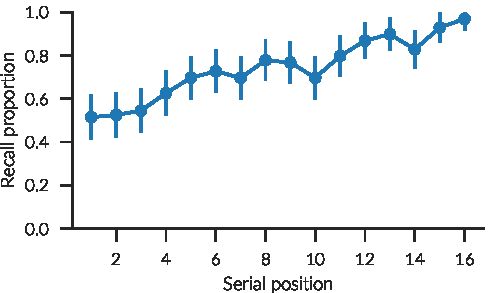
\includegraphics{figures/results/scopolamine-serial}
    \caption{Serial position curve with a scopolamine injection predicted by the CUE model}\label{fig:scopolamine-serial}
\end{figure} 


\section{Hebb repetition effect}
TODO


\section{Memory encoding}
As a spiking neural network model, the CUE model allows the recording of spikes and examination of changes in neural firing (\cref{fig:spikes}).
The distribution of active neurons changes for the STM neurons with each item, with a delay of about \SI{250}{\milli\second} to encode the new item.
When no new item is present, persistent neural firing preserves the firing pattern.
Similar behaviour is observed for neurons encoding the current context signal that gets updated with about a \SI{100}{\milli\second} delay.
The LTM for $\mtf$ (and $\mft$, but not shown) is encoded in neural weights that change for each list item to encode the newly learned associations.
\begin{figure}
    \centering
    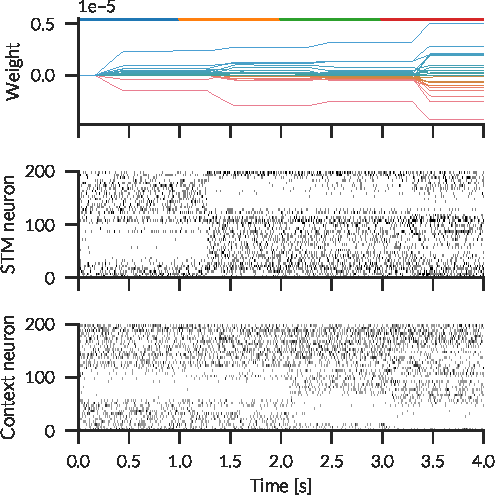
\includegraphics{figures/spikes}
    \caption[Memory encoding in the CUE model]{Memory encoding in the CUE model. From top to bottom: weights encoding $\mtf$ in LTM, spiking activity of a subset of STM neurons, and spiking activity of a subset of neurons encdoing the context signal $\ctx$. The colored bars at the top mark the presentation of four list different list items.}\label{fig:spikes}
\end{figure}
